% This is LLNCS.DEM the demonstration file of
% the LaTeX macro package from Springer-Verlag
% for Lecture Notes in Computer Science,
% version 2.4 for LaTeX2e as of 16. April 2010
%
\documentclass{llncs}
%
\usepackage{makeidx}  % allows for indexgeneration
\usepackage{color} %vrivas, 15-Jan-2016
\usepackage{hyperref} %vrivas, 21-Jan-2016, for \url
\usepackage{graphicx} %vrivas, 27-Jan-2016, for images
\usepackage{listings}%vrivas, 27-Jan-2016, for code
%c
\begin{document}
%
\frontmatter          % for the preliminaries
%
\pagestyle{headings}  % switches on printing of running heads
\addtocmark{Web browser-based forecasting} % additional mark in the TOC
%
%\chapter*{Preface}
%%
%This textbook is intended for use by students of physics, physical
%chemistry, and theoretical chemistry. The reader is presumed to have a
%basic knowledge of atomic and quantum physics at the level provided, for
%example, by the first few chapters in our book {\it The Physics of Atoms
%and Quanta}. The student of physics will find here material which should
%be included in the basic education of every physicist. This book should
%furthermore allow students to acquire an appreciation of the breadth and
%variety within the field of molecular physics and its future as a
%fascinating area of research.
%
%For the student of chemistry, the concepts introduced in this book will
%provide a theoretical framework for that entire field of study. With the
%help of these concepts, it is at least in principle possible to reduce
%the enormous body of empirical chemical knowledge to a few basic
%principles: those of quantum mechanics. In addition, modern physical
%methods whose fundamentals are introduced here are becoming increasingly
%important in chemistry and now represent indispensable tools for the
%chemist. As examples, we might mention the structural analysis of
%complex organic compounds, spectroscopic investigation of very rapid
%reaction processes or, as a practical application, the remote detection
%of pollutants in the air.

%\vspace{1cm}
%\begin{flushright}\noindent
%April 1995\hfill Walter Olthoff\\
%Program Chair\\
%ECOOP'95
%\end{flushright}
%%
%\chapter*{Organization}
%ECOOP'95 is organized by the department of Computer Science, Univeristy
%of \AA rhus and AITO (association Internationa pour les Technologie
%Object) in cooperation with ACM/SIGPLAN.
%%
%\section*{Executive Commitee}
%\begin{tabular}{@{}p{5cm}@{}p{7.2cm}@{}}
%Conference Chair:&Ole Lehrmann Madsen (\AA rhus University, DK)\\
%Program Chair:   &Walter Olthoff (DFKI GmbH, Germany)\\
%Organizing Chair:&J\o rgen Lindskov Knudsen (\AA rhus University, DK)\\
%Tutorials:&Birger M\o ller-Pedersen\hfil\break
%(Norwegian Computing Center, Norway)\\
%Workshops:&Eric Jul (University of Kopenhagen, Denmark)\\
%Panels:&Boris Magnusson (Lund University, Sweden)\\
%Exhibition:&Elmer Sandvad (\AA rhus University, DK)\\
%Demonstrations:&Kurt N\o rdmark (\AA rhus University, DK)
%\end{tabular}
%%
%\section*{Program Commitee}
%\begin{tabular}{@{}p{5cm}@{}p{7.2cm}@{}}
%Conference Chair:&Ole Lehrmann Madsen (\AA rhus University, DK)\\
%Program Chair:   &Walter Olthoff (DFKI GmbH, Germany)\\
%Organizing Chair:&J\o rgen Lindskov Knudsen (\AA rhus University, DK)\\
%Tutorials:&Birger M\o ller-Pedersen\hfil\break
%(Norwegian Computing Center, Norway)\\
%Workshops:&Eric Jul (University of Kopenhagen, Denmark)\\
%Panels:&Boris Magnusson (Lund University, Sweden)\\
%Exhibition:&Elmer Sandvad (\AA rhus University, DK)\\
%Demonstrations:&Kurt N\o rdmark (\AA rhus University, DK)
%\end{tabular}
%%
%\begin{multicols}{3}[\section*{Referees}]
%V.~Andreev\\
%B\"arwolff\\
%E.~Barrelet\\
%H.P.~Beck\\
%G.~Bernardi\\
%E.~Binder\\
%P.C.~Bosetti\\
%Braunschweig\\
%F.W.~B\"usser\\
%T.~Carli\\
%A.B.~Clegg\\
%G.~Cozzika\\
%S.~Dagoret\\
%Del~Buono\\
%P.~Dingus\\
%H.~Duhm\\
%J.~Ebert\\
%S.~Eichenberger\\
%R.J.~Ellison\\
%Feltesse\\
%W.~Flauger\\
%A.~Fomenko\\
%G.~Franke\\
%J.~Garvey\\
%M.~Gennis\\
%L.~Goerlich\\
%P.~Goritchev\\
%H.~Greif\\
%E.M.~Hanlon\\
%R.~Haydar\\
%R.C.W.~Henderso\\
%P.~Hill\\
%H.~Hufnagel\\
%A.~Jacholkowska\\
%Johannsen\\
%S.~Kasarian\\
%I.R.~Kenyon\\
%C.~Kleinwort\\
%T.~K\"ohler\\
%S.D.~Kolya\\
%P.~Kostka\\
%U.~Kr\"uger\\
%J.~Kurzh\"ofer\\
%M.P.J.~Landon\\
%A.~Lebedev\\
%Ch.~Ley\\
%F.~Linsel\\
%H.~Lohmand\\
%Martin\\
%S.~Masson\\
%K.~Meier\\
%C.A.~Meyer\\
%S.~Mikocki\\
%J.V.~Morris\\
%B.~Naroska\\
%Nguyen\\
%U.~Obrock\\
%G.D.~Patel\\
%Ch.~Pichler\\
%S.~Prell\\
%F.~Raupach\\
%V.~Riech\\
%P.~Robmann\\
%N.~Sahlmann\\
%P.~Schleper\\
%Sch\"oning\\
%B.~Schwab\\
%A.~Semenov\\
%G.~Siegmon\\
%J.R.~Smith\\
%M.~Steenbock\\
%U.~Straumann\\
%C.~Thiebaux\\
%P.~Van~Esch\\
%from Yerevan Ph\\
%L.R.~West\\
%G.-G.~Winter\\
%T.P.~Yiou\\
%M.~Zimmer\end{multicols}
%%
%\section*{Sponsoring Institutions}
%%
%Bernauer-Budiman Inc., Reading, Mass.\\
%The Hofmann-International Company, San Louis Obispo, Cal.\\
%Kramer Industries, Heidelberg, Germany
%
%%
%\tableofcontents
%
\mainmatter              % start of the contributions
%
\title{Web browser-based forecasting of economic time-series}
%
\titlerunning{Web browser-based forecasting}  % abbreviated title (for running head)
%                                     also used for the TOC unless
%                                     \toctitle is used
%
\author{
V. M. Rivas\inst{1}
\and Other?\inst{2}
}
%
\authorrunning{V. M. Rivas et al.} % abbreviated author list (for running head)
%
%%%% list of authors for the TOC (use if author list has to be modified)
\tocauthor{V M. Rivas}
%
%\institute{Depto. de Informatica, Univ. de Jaen, SPAIN,\\
\institute{Universidad de Ja\'{e}n, Department of Computer Sciences,\\
Campus Las Lagunillas s/n, 23071, Ja\'{e}n, SPAIN\\
\email{vrivas@ujaen.es},\\
\texttt{http://vrivas.es}
\and
%Depto. de Arquitectura y Tecnolog\'{\i}as de las Computadoras\\
%Univ. de Granada, SPAIN
Department of Computers, Architecture and Technology,\\
C/ Periodista Daniel Saucedo s/n, 18071, Granada, SPAIN
}

\maketitle              % typeset the title of the contribution
\textbf{Selling point: Economic time-series (currency exchange) can be forecasted using web browser while user are reading the content of a web-page. Lot of clients running simultaneously can lead to find very good solutions.}
\begin{abstract}
{\color{red}
The abstract should summarize the contents of the paper
using at least 70 and at most 150 words. It will be set in 9-point
font size and be inset 1.0 cm from the right and left margins.
There will be two blank lines before and after the Abstract. \dots
}
\keywords{Time-series forecasting, evolutionary computation, radial basis function neural networks, Web-based programming, volunteer computation}
\end{abstract}
%
\section{Introduction}
% Web-based computing
Web browsers stopped to be just simple HTML renders at the moment they allowed the executions of third-part programs included in the pages they downloaded. This way, browsers turned into wider frameworks in which multi-platform applications could be ran. Flash??? reference??? and Java applets reference??? are probably the best known techniques to do this, even for non-experts users. But, in fact, most of the code currently executed by browsers is written in a language called JavaScript reference???. The web, as we currently use it, would not be the same without the capability that JavaScript gives to the browser to make calculus, interact with the user, or dynamically retrieve data from servers without reloading the whole page, as it's done with AJAX Reference???.

% Historia de JavaScript???

% Restricciones de JavaScript
JavaScript is a general-purpose, object-based, event-driven language, that can be used to write programs for both the server and the client. The way developers can add JavaScript code to their web pages or web applications is relatively simple: the code is inserted in the HTML code in plain text, being later interpreted and executed by the browser itself, once having being downloaded from the server. A vast majority (if not all) of nowadays, everyday, massively-used web pages and applications (including those related to social networks) exist thanks to this language. Thus, although web browsers allow the users to change the preferences in order to disable the execution of any JavaScript code, this is rarely done in these days. Even more, most standard web users are not aware of the existence of this language, not realizing their browsers are working as programming environments in which code is analyzed, translated into a low-level language and executed. Consequently, and for safety reasons, programs written in JavaScript are executed in browsers using a sandbox model. This model imposes a series of restriction that could be summarized as: the JavaScript program inserted in a given web page cannot access any other resources that the ones contained in that web page. JavaScript programs can also access to the client's disk in order to store little pieces of text (called cookies), and also when the user has to select a file to be sent across the net.

Due to the capabilities of JavaScript, in this work we propose the use of web browsers as agents able to download a set of data, execute an evolutionary algorithm that evolves neural nets, and apply this neural nets to forecast an economic time-series. Using this approach, any of the huge amount of devices in the world able to execute a web browser (from computers to smart TVs, including smart phones) can be used to run our algorithm, contributing to find new solutions.

% Genetic Algorithms and RBFNN
Both the problem being considered in this paper and the algorithms used to solve it were introduced in \cite{Rivas04}. On the one hand, the problem consist on forecasting the values of the
exchange rates between two currencies, for a four years period (data is weekly averaged). On the other hand, the algorithm (described in section \ref{sec:algorithm} is a reduced version of {\em EvRBF} (\cite{Rivas04}), an evolutionary algorithm that makes Radial Basis Function Neural Networks (RBFNN) to evolve.

RBFNN are feed-forward neural nets with just one hidden and one output layer Reference???. The neurons in the output layer (only one neuron in this work) compute a weighted sum using outputs provided by hidden neurons, multiplied by some weights previously established, and adding a bias. The neurons in the hidden layer receive the input samples concerning the problem being resolved, and apply an activation function that  is a Radial Basis Function, i.e., a function returning a value that depends on the distance from the input values to a pre-established center of the function. The shape of this function is modified by means of a radius or width: the narrower this width, the higher the number of inputs that will not activate the neuron. Usually, Gaussian function is selected as the activation function, but many others can also be used.

Configuring an RBFNN in order to solve a task consist on: a) choosing the activation function for hidden neurons, b) choosing the correct number of hidden and output neurons, c) setting the parameters needed to apply the activation functions (i.e., center and radius), and d) setting the values for weights and bias. In any case, this last step can be easily computed once the rest of components have been established. Actually, the best set of weights and the bias can be computed using the Least Mean Square method.Taking this into account, the {\em EvRBF} algorithm has been designed to automatically search for the best configuration of an RBFNN that solves the problem being faced, except for the activation function to be used (i.e, the RBF) that is set a priori.

% Time-series prediction
RBFNN have being successfully used by researchers to solve problems like classification, function approximation, and, as in this work, time-series forecasting \cite{Broomhead88,Keogh03,Whitehead}. Time-series can be considered as a special kind of function approximation where future values of the series are expressed as a function of past ones. There exist many methods in literature developed to forecast time-series references???, being ARIMA \cite{BoxJenk} probably the most widely used.

In the herein, the implementation of {\em EvRBF} for web browsers (called {\em jsEvRBF}) has been compared to its original implementation as well as to the method by REFERENCE, the one introducing the time-series tackled in this paper. The paper has been organized in the following sections: section \ref{sec:algorithm} describes our algorithm; section \ref{sec:experiments} describes the problem to which the algorithm has been applied, as well as the experiments carried out and the results yielded. Finally, we draw some conclusions in section \ref{sec:conclusions}, and propose some future lines.


\section{The {\em jsEvRBF} algorithm}
\label{sec:algorithm}
% The {\em EvRBF} general skeleton
{\em jsEvRBF} is an evolutionary algorithm written in JavaScript, so that it can be executed in web browsers.  As its predecessor \cite{Rivas04}, its main characteristic is that individuals are complete RBFNN; for this reason, special operators have been programmed in order to cross and mutate this kind of networks. Apart from this, it is a generational algorithm, with a fixed number of individuals, and uses tournament selection and elitist replacement. The code can be downloaded or forked from \url{http://bit.ly/jsEvRBF}; its use is restricted under the terms of the Apache 2.0 license.

In order to implement both the RBFNN and the evolutionary algorithm, two JavaScript libraries have been developed by our research group, namely {\em jsRBFNN}\footnote{\url{http://bit.ly/jsRBFNN}} and {\em jsEO}\footnote{\url{http://bit.ly/js-EO}}. The first one implements the nets and also the LMS training algorithm to get the weights once a net has been built. The second one, {\em jsEO} REFRENCE-EVOSTAR??? is a more complex framework that allows the generation of many kinds of evolutionary algorithms, making easier the task of creating new kind of individuals and operators by means of inheritance (as defined in object-oriented programming). Figure \ref{fig:class_diagram} graphically shows the set of dependencies between the algorithm and the rest of libraries. 


As a standard evolutionary algorithm, the skeleton of jsEvRBF is the following:


\begin{lstlisting}
(1) Create, train and evaluate an initial population \
        of _p_ individuals.
(2) During _n_ generations do:
   (2.1) Select a subpopulation of _q_ individuals
   (2.2.) Create _q_ new individuals applying an operator \
          to any of the ones in subpopulation
   (2.3) Train and evaluate the _q_ new individuals
   (2.4) Join and sort both old and new populations
   (2.5) Remove the _q_ worst individuals
(3) Send the forecasting done by the best individual \
   in last generation to the server
\end{lstlisting}


\begin{figure}[!ht]
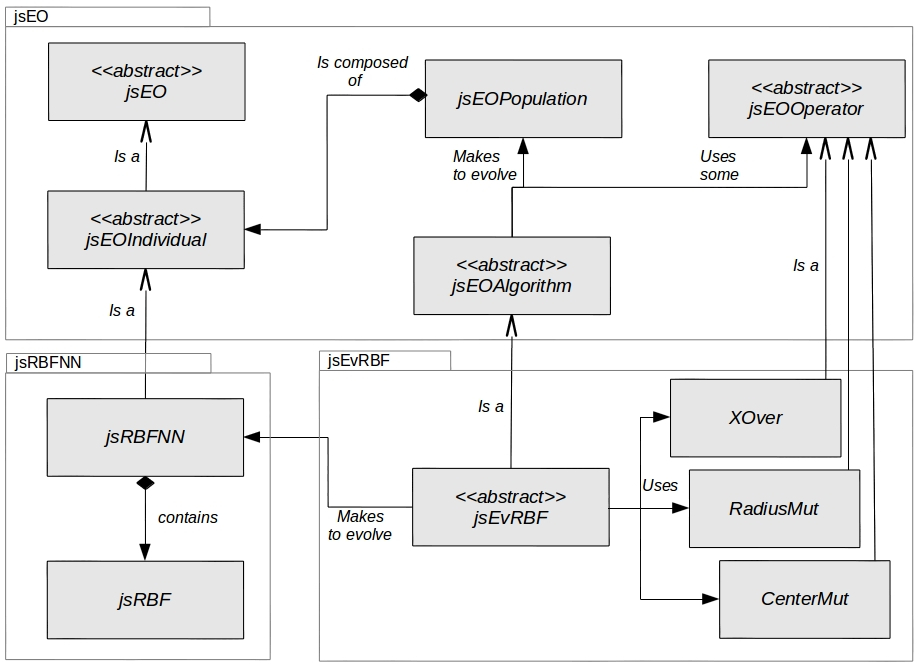
\includegraphics[width=120mm]{class-diagram.jpg}
\caption{Class diagram of the jsEvRBF algorithm, showing the way it depends on the jsEO general framework and the jsRBFNN library.}
\label{fig:class_diagram}
\end{figure}


The individuals are RBFNN, any of them composed of a set of hidden neurons implemented as a vector of objects. Every hidden neuron stores its center and radius, and the global RBFNN stores the weights and bias. 

With respect to the operators used in this algorithm:

\begin{itemize}
\item {\em XOver.} Takes two individuals as inputs and operates by randomly selecting a set of neurons from first individual and another set (probably of a different size) from the second one. After this, those sets are interchanged.

\item {\em CenterMut.} Modifies a percentage of the centers of the individual it gets as input, just setting the new center to random values in the range defined by the input dimension.

\item {\em RadiusMut.} Quite similar to the precendent, this operator modifies a percentage of the radius of the neurons belonging to the individual received, choosing a new value in the same way the {\em CenterMut} operators does.
\end{itemize}



3.1. Binary cross-over operator
The binary-operator needs two RBF NNs to be applied, although it only
changes one of them. This operator takes an uniformly random chosen number
of consecutive hidden neurons from the first network, and another random
sequence from the second; then it replaces the first of these sequences by the
second one, so that the second individual remains unchanged.
3.2. Unary operators
Given that in a RBF NN the optimum weights from hidden-to-output
neurons can be easily computed, the unary or mutation-like operators affect the
hidden neuron components, centers and radii, in their quantities and values,
but not the hidden-to-output weights.
Centers mutator. This operator changes a given percentage of the compo-
nents of the center of every hidden neuron. Each component of the center
is modified by adding or subtracting a random value, which is chosen fol-
lowing a Gaussian probability function with mean 0 and standard deviation
0.1.
Radii mutator. This operator is applied to one of the existing nets, but affects
to the radii of the RBF. Radii are modified using a Gaussian function as de-
fined previously. Radi

% Specific characteristics of this implementation
% Operators
\section{Experiments and results}
\label{sec:experiments}
% The data-set
% Two kind of experiments?
% First one: lot of different browsers, short executions
% Second one: only one browser, complete executions
% Comparisons between them and original papers
\section{Conclusions}
\label{sec:conclusions}
% It's possible to do, although some improvements have to be done, like migration
% computation can be done while users are reading/using a web page
% Servers need to have great computational power, but only the needed to serve many different problems, and store the information sent by clients.

\section*{Acknowledges}
%
% ---- Bibliography ----
%
\begin{thebibliography}{}
%
%\bibitem[1980]{2clar:eke}
%Clarke, F., Ekeland, I.:
%Nonlinear oscillations and
%boundary-value problems for Hamiltonian systems.
%Arch. Rat. Mech. Anal. 78, 315--333 (1982)

\bibitem[1]{BoxJenk}
Box, G.E., Jenkins G.M.: Time series analysis: forecasting and control. San Francisco: Holden Day (1976)

\bibitem[2]{Broomhead88}
Broomhead, D.S., Lowe D.: Multivariable functional interpolation and adaptive networks. Complex Systems, 2, 321--355 (1988)

\bibitem[3]{Keogh03}
Keogh, E.: On the Need for Time Series Data Mining Benchmarks: A Survey and Empirical. Data Mining and Knowledge Discovery, 7(4), 349--371 (2003).

%\bibitem[4]{Pena2005}
%Pe�a D.: An\'alisis de Series Temporales, Alianza Editorial, ISBN 84-206-9128-3 (2005)
   
\bibitem[5]{Rivas04}
Rivas, V.M., Merelo, J.J., Castillo, P.A., Arenas, M.G., Castellanos, J.G.: Evolving RBF neural networks for time-series forecasting with EvRBF. Information Sciences, 165(3-4), 207--220 (2004)

\bibitem[6]{Whitehead}
Whitehead, B., Choate, T.: Cooperative-competitive genetic evolution of Radial Basis Function centers and widths for time series predictioN. IEEE Trans. on Neural Networks, 7(4), 869--880 (1996).


   
\end{thebibliography}
%\clearpage
%\addtocmark[2]{Author Index} % additional numbered TOC entry
%\renewcommand{\indexname}{Author Index}
%\printindex
%\clearpage
%\addtocmark[2]{Subject Index} % additional numbered TOC entry
%\markboth{Subject Index}{Subject Index}
%\renewcommand{\indexname}{Subject Index}
%\input{subjidx.ind}
\end{document}
